\documentclass[12pt,a4paper]{article}

%% ── Packages ──────────────────────────────────────────────────────────────
\usepackage[margin=2.5cm]{geometry}
\usepackage{fontenc}
\usepackage{inputenc}
\usepackage[T1]{fontenc}
\usepackage{lmodern}
\usepackage{microtype}
\usepackage{graphicx}
\usepackage{booktabs}
\usepackage{multirow}
\usepackage{tabularx}
\usepackage{longtable}
\usepackage{array}
\usepackage{xcolor}
\usepackage{amsmath,amssymb}
\usepackage{listings}
\usepackage{hyperref}
\usepackage{caption}
\usepackage{subcaption}
\usepackage{float}
\usepackage{parskip}
\usepackage{fancyhdr}
\setlength{\headheight}{13.6pt}
\usepackage{titlesec}
\usepackage{enumitem}
\usepackage{siunitx}
\usepackage{tikz}
\usetikzlibrary{shapes.geometric,arrows.meta,positioning,calc}

\sisetup{group-separator={,},group-minimum-digits=4}

%% ── Colors ───────────────────────────────────────────────────────────────
\definecolor{codeblue}{RGB}{30,100,200}
\definecolor{codegray}{RGB}{100,100,100}
\definecolor{codegreen}{RGB}{0,128,0}
\definecolor{codebg}{RGB}{248,248,248}
\definecolor{accentblue}{RGB}{25,84,166}
\definecolor{accentgray}{RGB}{80,80,80}

%% ── Listings (code) ──────────────────────────────────────────────────────
\lstdefinestyle{pycode}{
  language=Python,
  backgroundcolor=\color{codebg},
  basicstyle=\ttfamily\small,
  keywordstyle=\color{codeblue}\bfseries,
  commentstyle=\color{codegreen}\itshape,
  stringstyle=\color{orange},
  numberstyle=\tiny\color{codegray},
  numbers=left,
  numbersep=8pt,
  stepnumber=1,
  frame=single,
  framerule=0.5pt,
  rulecolor=\color{gray!40},
  tabsize=4,
  showstringspaces=false,
  breaklines=true,
  breakatwhitespace=true,
  captionpos=b,
  xleftmargin=15pt,
  aboveskip=8pt,
  belowskip=8pt,
}
\lstset{style=pycode}

%% ── Headers / Footers ────────────────────────────────────────────────────
\pagestyle{plain}
\fancyhf{}
\fancyhead[L]{\small\color{accentgray} AdaptiveTile: EDA \& Prototype Report}
\fancyhead[R]{\small\color{accentgray} Humaira Ayesha --- 23301683}
\fancyfoot[C]{\small\thepage}
\renewcommand{\headrulewidth}{0.4pt}

%% ── Section Formatting ───────────────────────────────────────────────────
\titleformat{\section}{\large\bfseries\color{black}}{%
  \thesection}{1em}{}
\titleformat{\subsection}{\normalsize\bfseries\color{accentgray}}{\thesubsection}{1em}{}
\titleformat{\subsubsection}{\normalsize\itshape\color{accentgray}}{\thesubsubsection}{1em}{}

%% ── Hyperlinks ────────────────────────────────────────────────────────────
\hypersetup{
  colorlinks=true,
  linkcolor=black,
  urlcolor=accentblue,
  citecolor=accentblue,
  pdftitle={AdaptiveTile: EDA and Prototype Report},
  pdfauthor={Humaira Ayesha},
}

%% ── Graphics Path ────────────────────────────────────────────────────────
\graphicspath{%
  {../adaptive-tile-processing/outputs/figures/}%
  {../adaptive-tile-processing/outputs/plots/}%
}

%% ─────────────────────────────────────────────────────────────────────────
\begin{document}

%% ── Title Page ───────────────────────────────────────────────────────────
\begin{titlepage}
  \centering
  \vspace*{2cm}

  {\LARGE\bfseries\color{black}
    AdaptiveTile:\\[0.3em]
    Content-Aware Parallel Image Processing\\[0.3em]
    with Predictive Tile Scheduling
  \par}

  \vspace{1.5cm}

  {\large\bfseries EDA \& Prototype Submission Report\par}

  \vspace{0.5cm}
  \rule{0.6\textwidth}{0.4pt}
  \vspace{0.5cm}

  {\large
    \textbf{Author:} Humaira Ayesha\\[0.3em]
    \textbf{Student ID:} 23301683\\[0.3em]
    \textbf{Course:} PARALLEL, DISTRIBUTED, AND HIGH-PERFORMANCE COMPUTING\\[0.3em]
    \textbf{Institution:} Brac University, Department of Computer Science and Engineering\\[0.3em]
    \textbf{Date:} 5 May 2026
  \par}

  \vspace{1.5cm}

  \vfill

  {\small Brac University, Department of Computer Science and Engineering\\
    Bangladesh --- 2026}
\end{titlepage}

\thispagestyle{fancy}
\tableofcontents
\newpage

%% ==========================================================================
\section{Project Overview}
%% ==========================================================================

AdaptiveTile is an end-to-end system for content-aware parallel image processing.
Its central insight is that image tiles are not computationally uniform: tiles containing rich textures, sharp edges, or complex gradients take significantly longer to process than smooth, featureless regions.
Conventional static work allocation ignores this heterogeneity, causing load imbalance and degraded parallel efficiency.
AdaptiveTile addresses this by predicting per-tile compute cost from content features and using those predictions to schedule work more evenly across CPU and GPU workers.

\subsection{Research Objectives}

\begin{enumerate}[leftmargin=*]
  \item \textbf{Feature Engineering:} Extract lightweight per-tile content
        descriptors that correlate with processing time.

  \item \textbf{Complexity Prediction:} Train and compare machine learning regressors
        to predict per-tile processing time from those content features.

  \item \textbf{Adaptive Scheduling:} Evaluate four scheduling strategies---Static,
        Dynamic, Predictive, and Hybrid---on benchmark images.

  \item \textbf{CPU--GPU Evaluation:} Measure speedup, parallel efficiency,
        and output quality across four execution modes.

  \item \textbf{Generalisation:} Validate performance on three publicly available
        datasets: Kodak, DIV2K, and BSDS500.
\end{enumerate}

\subsection{System Architecture}

Figure~\ref{fig:arch} shows the high-level pipeline of AdaptiveTile.

\begin{figure}[!ht]
\centering
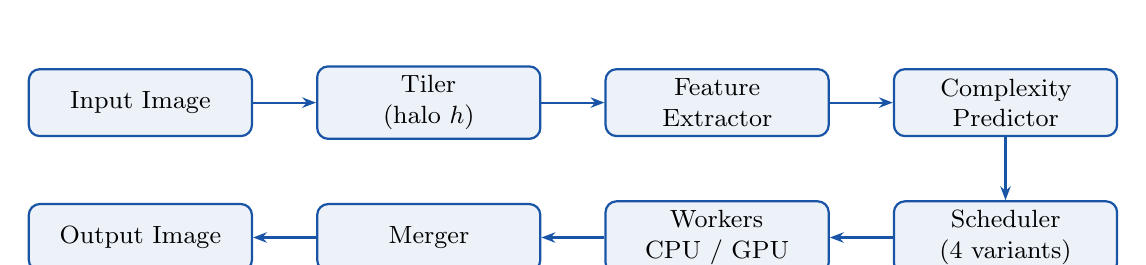
\begin{tikzpicture}[
  box/.style={rectangle, rounded corners=4pt, draw=accentblue, thick,
              fill=accentblue!8, text width=2.6cm, align=center,
              minimum height=0.85cm, font=\small},
  arr/.style={-{Stealth[length=5pt]}, thick, color=accentblue},
  font=\small
]
  \node[box] (img)   {Input Image};
  \node[box, right=0.8cm of img]   (tile)  {Tiler\\(halo $h$)};

  \node[box, right=0.8cm of tile]  (feat)  {Feature\\Extractor};
  \node[box, right=0.8cm of feat]  (pred)  {Complexity\\Predictor};
  \node[box, below=0.8cm of pred]  (sched) {Scheduler\\(4 variants)};
  \node[box, left=0.8cm of sched]  (work)  {Workers\\CPU / GPU};
  \node[box, left=0.8cm of work]   (merge) {Merger};
  \node[box, left=0.8cm of merge]  (out)   {Output Image};

  \draw[arr] (img)   -- (tile);
  \draw[arr] (tile)  -- (feat);
  \draw[arr] (feat)  -- (pred);
  \draw[arr] (pred)  -- (sched);
  \draw[arr] (sched) -- (work);
  \draw[arr] (work)  -- (merge);
  \draw[arr] (merge) -- (out);
\end{tikzpicture}
\caption{AdaptiveTile system architecture: tiling $\to$ feature extraction
$\to$ complexity prediction $\to$ scheduling $\to$ parallel execution $\to$ merging.}
\label{fig:arch}
\end{figure}

\subsection{Datasets}

Three publicly available benchmark datasets are used:

\begin{table}[!ht]
\centering
\small
\caption{Dataset summary.}
\label{tab:datasets}
\begin{tabular}{llrrl}
\toprule
\textbf{Dataset} & \textbf{Resolution} & \textbf{Images} & \textbf{Format} & \textbf{Role} \\
\midrule
Kodak   & $768\times512$ / $512\times768$ & 24  & PNG & Primary profiling \& benchmarking \\

DIV2K   & $\approx2048\times1080$         & 900 & PNG & Generalisation (high-res) \\
BSDS500 & $481\times321$                  & 500 & JPG & Generalisation (low-res) \\

\bottomrule
\end{tabular}
\end{table}

Default experimental parameters: tile size $s=128$\,px, halo $h=16$\,px,
workers $W\in\{1,2,4,6,8\}$, GPU streams $S=4$.

%% ==========================================================================
\section{Exploratory Data Analysis (EDA)}
%% ==========================================================================

\subsection{Tile Profiling Procedure}

We tile all 24 Kodak images with $s=128$\,px and halo $h=16$\,px, yielding a $4\times6$ grid of 24 tiles per image---576 tiles in total.
Each tile is processed three times through Pipeline~B (denoise threshold), and the median runtime is recorded to offset system jitter.
This produces a dataset of 576 observations, each comprising seven content features, spatial indices (row and column), and a runtime target in milliseconds.

\subsection{Target Variable: Per-Tile Runtime}

\begin{table}[!ht]
\centering
\small
\caption{Descriptive statistics of per-tile runtime (ms), 576 raw tiles.}
\label{tab:runtime_stats}
\begin{tabular}{lr}
\toprule
\textbf{Statistic} & \textbf{Value} \\
\midrule
Minimum   & 0.159 ms \\
Maximum   & 0.668 ms \\
Mean      & 0.317 ms \\
Std Dev   & 0.084 ms \\
CV        & 26.55\% \\
Skewness  & 0.89 \\
Kurtosis  & 0.97 \\
Normality & Non-normal ($p<0.001$, Shapiro-Wilk) \\

\bottomrule
\end{tabular}
\end{table}

A coefficient of variation of $26.55\%$ confirms that tile complexity varies enough to make prediction worthwhile---uniform tiles would show near-zero CV and leave no room for scheduling gains.

\begin{figure}[!ht]
\centering

\includegraphics[width=0.95\textwidth]{eda_07_target_analysis.png}
\caption{Per-tile runtime distribution. Right-skewed histogram and Q-Q plot
confirming non-normality.}
\label{fig:target_dist}
\end{figure}

\subsection{Feature Distributions}

We extract seven content features per tile to capture its visual complexity.

\begin{table}[!ht]
\centering
\small
\caption{Summary statistics for all features (576 raw tiles).}
\label{tab:feat_stats}
\begin{tabular}{lrrrrl}
\toprule
\textbf{Feature} & \textbf{Mean} & \textbf{Std} & \textbf{Skew} & \textbf{Kurt} & \textbf{Normal?} \\
\midrule
Edge density       & 0.147  & 0.098  & 0.23  & -0.87 & No \\
Gradient variance  & 7211.6 & 6779.6 & 1.73  & 2.87  & No \\
Intensity variance & 1523.9 & 1473.9 & 2.33  & 5.41  & No \\
Histogram entropy  & 1.825  & 0.492  & -1.00 & 0.08  & No \\
LBP texture score  & 5.184  & 0.354  & 2.41  & 6.29  & No \\
\bottomrule
\end{tabular}
\end{table}

\begin{figure}[!ht]
\centering

\includegraphics[width=\linewidth,height=0.85\textheight,keepaspectratio]{eda_01_distributions.png}
\caption{Feature distributions for 576 raw tiles (3x3 grid).}
\label{fig:feat_dist}
\end{figure}

\subsection{Outlier Detection}

A majority-vote ensemble of three rules (IQR, MAD, and $3\sigma$) flags a tile as an outlier when at least two agree.
This removes \textbf{64 tiles (11.1\%)}, leaving 512 clean tiles for model training and evaluation.

\begin{figure}[!ht]
\centering

\includegraphics[width=0.98\textwidth]{eda_02_outliers.png}
\caption{Outlier detection across all features. Flagged tiles shown in red.}
\label{fig:outliers}
\end{figure}

\subsection{Feature--Runtime Correlation}

\begin{table}[H]
\centering
\caption{Pearson and Spearman correlation of features with runtime ($p<0.001$).}
\label{tab:corr}
\begin{tabular}{lrr}
\toprule
\textbf{Feature}    & \textbf{Pearson $r$} & \textbf{Spearman $\rho$} \\

\midrule
Histogram entropy   & +0.445 & +0.471 \\
Edge density        & +0.439 & +0.488 \\
Gradient variance   & +0.400 & +0.493 \\
Intensity variance  & +0.197 & +0.357 \\
LBP texture score   & -0.359 & -0.411 \\
Tile row            & +0.074 & +0.119 \\
Tile col            & -0.078 & -0.053 \\
\bottomrule
\end{tabular}
\end{table}

\begin{figure}[!ht]
\centering

\includegraphics[width=0.95\textwidth]{eda_03_correlation_heatmaps.png}
\caption{Pearson, Spearman, and Kendall correlation heatmaps.}
\label{fig:corr}
\end{figure}

\subsection{Train/Test Distributional Shift}

\begin{table}[H]
\centering
\caption{Train/test distributional shift (PSI $>0.2$ = significant).}

\label{tab:drift}
\begin{tabular}{lrrl}
\toprule
\textbf{Feature}   & \textbf{PSI} & \textbf{JSD} & \textbf{Drift?} \\
\midrule
Edge density       & 0.133 & 0.044 & No \\
Gradient variance  & 0.052 & 0.026 & No \\
Intensity variance & 0.170 & 0.034 & No \\
Histogram entropy  & 0.229 & 0.061 & \textbf{Yes} \\
LBP texture score  & 0.223 & 0.034 & \textbf{Yes} \\
Runtime (ms)       & 0.254 & 0.054 & \textbf{Yes} \\
\bottomrule
\end{tabular}
\end{table}

\begin{figure}[!ht]
\centering

\includegraphics[width=0.98\textwidth]{eda_04_train_test_distributions.png}
\caption{Train vs.\ test feature distributions (GroupShuffleSplit 80/20).}
\label{fig:drift}
\end{figure}

\subsection{Dimensionality Reduction}

\begin{figure}[!ht]
\centering

\includegraphics[width=0.98\textwidth]{eda_05_dimensionality_reduction.png}
\caption{Left: PCA (6 components = 95\% variance). Right: t-SNE showing three
runtime clusters (fast, medium, slow tiles).}
\label{fig:dimred}
\end{figure}

\subsection{Preprocessing Pipeline Summary}

EDA findings motivate a three-step preprocessing pipeline:
(1) majority-vote outlier removal (64 tiles, 11.1\%);
(2) Yeo--Johnson power transformation to reduce skewness in gradient and intensity features;
(3) RobustScaler normalisation to limit the influence of remaining heavy tails.

\begin{figure}[!ht]
\centering

\includegraphics[width=0.95\textwidth]{eda_08_before_after_preprocessing.png}
\caption{Feature distributions before and after preprocessing.}
\label{fig:preproc}
\end{figure}

%% ==========================================================================
\section{Prototype Implementation}
%% ==========================================================================

The prototype implements the full AdaptiveTile pipeline in Python, end-to-end:
tiling with halo borders, feature extraction, complexity prediction, scheduling,
parallel CPU and GPU execution, and tile merging.

\subsection{Module Structure}

\begin{table}[H]
\centering
\caption{Source module overview.}
\label{tab:modules}
\begin{tabular}{lp{9cm}}
\toprule
\textbf{Module} & \textbf{Responsibility} \\
\midrule
\texttt{src/config.py}      & Central configuration (tile size, halo, pipeline params) \\
\texttt{src/tiling.py}      & Extract tiles with halo borders from an image \\
\texttt{src/features.py}    & Compute 7 content features per tile \\
\texttt{src/predictor.py}   & Train and evaluate tabular + CNN complexity predictors \\
\texttt{src/scheduler.py}   & Static, Dynamic, Predictive, Hybrid schedulers \\
\texttt{src/worker\_cpu.py} & CPU processing pipelines A and B \\
\texttt{src/worker\_gpu.py} & GPU (Kornia) processing pipeline \\
\texttt{src/merge.py}       & Stitch processed tiles back into full image \\
\texttt{src/metrics.py}     & Speedup, efficiency, imbalance ratio, PSNR, SSIM \\
\bottomrule
\end{tabular}
\end{table}

\subsection{Configuration}

All hyperparameters live in a single \texttt{src/config.py} module, keeping experiments reproducible and easy to modify:

\begin{lstlisting}[caption={Central configuration (\texttt{src/config.py}).}, label=lst:config]
TILE_SIZE      = 128          # default tile side length (pixels)
HALO           = 16           # halo border width (pixels)
NUM_WORKERS    = min(8, cpu_count())
NUM_GPU_STREAMS = 4

CANNY_LOW, CANNY_HIGH = 50, 150
BILATERAL_D, BILATERAL_SIGMA = 9, 75
NLM_H = 10
MORPH_KERNEL_A, MORPH_KERNEL_B = 5, 3

CNN_EPOCHS, CNN_BATCH_SIZE = 30, 32
CNN_LR, CNN_IMG_SIZE = 1e-4, 224

TILE_SIZES   = [128, 256, 512, 1024]
HALOS        = [4, 8, 16, 32]
WORKER_COUNTS = [1, 2, 4, 8]
\end{lstlisting}

\subsection{Tiling with Halo Borders}

The tiler decomposes an image into $n_r \times n_c$ tiles, each extended by a halo border of $h$ pixels on every side, clamped to the image boundary so edge tiles do not read outside the array:

\begin{lstlisting}[caption={Tile extraction with halo borders (\texttt{src/tiling.py}).}, label=lst:tiling]
@dataclass
class TileInfo:
    tile_id: int
    row: int; col: int
    x_start: int; y_start: int; x_end: int; y_end: int
    left_halo: int; top_halo: int
    right_halo: int; bottom_halo: int
    data: np.ndarray   # halo-padded pixel array

def extract_tiles(image: np.ndarray,
                  tile_size: int, halo: int) -> list[TileInfo]:
    h, w = image.shape[:2]
    tiles, tid = [], 0
    for r in range(math.ceil(h / tile_size)):
        for c in range(math.ceil(w / tile_size)):
            x0, y0 = c * tile_size, r * tile_size
            x1 = min(x0 + tile_size, w)
            y1 = min(y0 + tile_size, h)
            xs = max(0, x0 - halo);  ys = max(0, y0 - halo)
            xe = min(w, x1 + halo);  ye = min(h, y1 + halo)
            tiles.append(TileInfo(
                tile_id=tid, row=r, col=c,
                x_start=x0, y_start=y0, x_end=x1, y_end=y1,
                left_halo=x0-xs, top_halo=y0-ys,
                right_halo=xe-x1, bottom_halo=ye-y1,
                data=image[ys:ye, xs:xe],
            ))
            tid += 1
    return tiles
\end{lstlisting}

\subsection{Feature Extraction}

Seven features capture the visual complexity of each tile:

\begin{lstlisting}[caption={Per-tile feature extraction (\texttt{src/features.py}).}, label=lst:features]
def extract_features(tile_bgr: np.ndarray,
                     row: int, col: int) -> dict:
    gray = cv2.cvtColor(tile_bgr, cv2.COLOR_BGR2GRAY).astype(np.float32)

    # Edge density: fraction of Canny edge pixels
    edges = cv2.Canny(gray.astype(np.uint8), CANNY_LOW, CANNY_HIGH)
    edge_density = float(edges.mean() / 255.0)

    # Gradient variance: Sobel magnitude variance
    sx = cv2.Sobel(gray, cv2.CV_32F, 1, 0, ksize=3)
    sy = cv2.Sobel(gray, cv2.CV_32F, 0, 1, ksize=3)
    gradient_variance = float(np.sqrt(sx**2 + sy**2).var())

    # Intensity variance and histogram entropy
    intensity_variance = float(gray.var())
    hist, _ = np.histogram(gray, bins=16, range=(0, 256))
    histogram_entropy = float(scipy_entropy(hist / hist.sum() + 1e-10))

    # LBP texture score (uniform, P=8, R=1)
    lbp = local_binary_pattern(gray.astype(np.uint8),
                               P=8, R=1, method="uniform")
    lbp_texture_score = float(lbp.mean())

    return {
        "edge_density":      edge_density,
        "gradient_variance": gradient_variance,
        "intensity_variance":intensity_variance,
        "histogram_entropy": histogram_entropy,
        "lbp_texture_score": lbp_texture_score,
        "tile_row":          float(row),
        "tile_col":          float(col),
    }
\end{lstlisting}

\subsection{Complexity Predictor}

We train eight tabular regressors and three CNN regressors on the profiled tile dataset, selecting the best-performing model by Spearman $\rho$:

\begin{lstlisting}[caption={Tabular model registry (\texttt{src/predictor.py}).}, label=lst:predictor]
TABULAR_MODELS = {
    "linear":            LinearRegression(),
    "ridge":             Ridge(alpha=1.0),
    "svr":               Pipeline([("scaler", StandardScaler()),
                                   ("model", SVR(kernel="rbf", C=10))]),
    "random_forest":     RandomForestRegressor(
                             n_estimators=100, n_jobs=-1, random_state=42),
    "gradient_boosting": GradientBoostingRegressor(
                             n_estimators=100, random_state=42),
    "xgboost":           xgb.XGBRegressor(n_estimators=100, lr=0.1),
    "lightgbm":          lgb.LGBMRegressor(n_estimators=100, lr=0.1),
    "mlp":               Pipeline([("scaler", StandardScaler()),
                                   ("model", MLPRegressor(
                                       hidden_layer_sizes=(64, 32)))]),
}

def fit_tabular(self, X, y):
    best_rho = -1.0
    for name, model in TABULAR_MODELS.items():
        m = deepcopy(model).fit(X, y)
        rho = spearmanr(y, m.predict(X)).correlation
        if rho > best_rho:
            best_rho = rho
            self.best_tabular_model = name
            self._best_model = m
\end{lstlisting}

\subsection{Scheduler Variants}

\begin{lstlisting}[caption={Four scheduler classes (\texttt{src/scheduler.py}).}, label=lst:schedulers]
class StaticScheduler:
    def assign(self, tiles, n_workers):
        # Round-robin tile assignment
        batches = [[] for _ in range(n_workers)]
        for i, tile in enumerate(tiles):
            batches[i % n_workers].append(tile)
        return batches

class DynamicScheduler:
    def get_queue(self, tiles):
        # FIFO queue; workers pull tasks as they finish
        return sorted(tiles, key=lambda t: t.tile_id)

class PredictiveScheduler:
    def get_queue(self, tiles, predictions):
        # LPT: longest predicted tile dispatched first
        order = np.argsort(predictions)[::-1]
        return [tiles[i] for i in order]

class HybridScheduler:
    def get_initial_queue(self, tiles, predictions):
        # Predictive initial ordering
        for i, t in enumerate(tiles):
            self._predicted_times[t.tile_id] = float(predictions[i])
        return [tiles[i] for i in np.argsort(predictions)[::-1]]

    def record_completion(self, tile_id, predicted_ms, actual_ms):
        # Track prediction errors for online adaptation
        self._errors.append(abs(actual_ms - predicted_ms))
\end{lstlisting}

\subsection{CPU Processing Pipelines}

\begin{lstlisting}[caption={CPU pipelines A and B (\texttt{src/worker\_cpu.py}).}, label=lst:pipelines]
def process_tile_cpu_pipeline_a(tile_bgr):
    # Edge+gradient pipeline (~7 ms/tile). High complexity variance.
    gray    = cv2.cvtColor(tile_bgr, cv2.COLOR_BGR2GRAY)
    blurred = cv2.GaussianBlur(gray, (5, 5), 1.0)
    sx = cv2.Sobel(blurred, cv2.CV_32F, 1, 0, ksize=3)
    sy = cv2.Sobel(blurred, cv2.CV_32F, 0, 1, ksize=3)
    mag = cv2.normalize(cv2.magnitude(sx, sy),
                        None, 0, 255, cv2.NORM_MINMAX, cv2.CV_8U)
    combined = cv2.addWeighted(
        mag, 0.5, cv2.Canny(blurred, CANNY_LOW, CANNY_HIGH), 0.5, 0)
    return cv2.morphologyEx(combined, cv2.MORPH_CLOSE,
        np.ones((MORPH_KERNEL_A,)*2, np.uint8))

def process_tile_cpu_pipeline_b(tile_bgr):
    # Denoise+threshold pipeline (~317 ms/tile). Primary benchmark.
    gray = cv2.cvtColor(tile_bgr, cv2.COLOR_BGR2GRAY)
    bl   = cv2.bilateralFilter(
        gray, BILATERAL_D, BILATERAL_SIGMA, BILATERAL_SIGMA)
    dn   = cv2.fastNlMeansDenoising(bl, None, h=NLM_H)
    thr  = cv2.adaptiveThreshold(dn, 255,
        cv2.ADAPTIVE_THRESH_GAUSSIAN_C, cv2.THRESH_BINARY, 11, 2)
    k    = np.ones((MORPH_KERNEL_B,)*2, np.uint8)
    return cv2.dilate(cv2.morphologyEx(thr, cv2.MORPH_OPEN, k),
                      k, iterations=1)
\end{lstlisting}

%% ==========================================================================
\section{Predictor Evaluation (Prototype Results)}
%% ==========================================================================

\subsection{Model Comparison}

\begin{table}[H]
\centering
\caption{Predictor MAE and Spearman $\rho$ (5-fold CV, GroupShuffleSplit).
Best in \textbf{bold}.}
\label{tab:predictors}
\begin{tabular}{lrrrr}
\toprule
\multirow{2}{*}{\textbf{Model}} &
\multicolumn{2}{c}{\textbf{Raw}} &
\multicolumn{2}{c}{\textbf{Preprocessed}} \\
\cmidrule(lr){2-3}\cmidrule(lr){4-5}
& MAE & $\rho$ & MAE & $\rho$ \\
\midrule
Linear Regression & 0.0588 & 0.543 & 0.0165 & 0.534 \\
Ridge             & 0.0593 & 0.571 & 0.0165 & 0.535 \\
SVR (RBF)         & 0.0724 & 0.352 & 0.0189 & --- \\
Random Forest     & 0.0572 & 0.542 & \textbf{0.0153} & \textbf{0.584} \\
Gradient Boosting & 0.0593 & 0.533 & 0.0166 & 0.507 \\
XGBoost           & 0.0605 & 0.452 & 0.0164 & 0.520 \\
LightGBM          & 0.0598 & 0.482 & 0.0159 & 0.538 \\
MLP               & 0.0787 & 0.418 & 0.0533 & 0.212 \\
\midrule
SqueezeNet        & 0.2481 & -0.097 & --- & --- \\
MobileNetV3-Small & 0.1385 & 0.203  & --- & --- \\
EfficientNet-B0   & 0.0876 & 0.003  & --- & --- \\
\bottomrule
\end{tabular}
\end{table}

\begin{figure}[!ht]
\centering

\includegraphics[width=0.95\textwidth]{training_05_feature_importance.png}
\caption{Random Forest feature importances (mean decrease in impurity). Edge
density and histogram entropy are the strongest predictors.}
\label{fig:feat_imp}
\end{figure}

\begin{figure}[!ht]
\centering

\includegraphics[width=0.95\textwidth]{training_03_predicted_vs_actual.png}
\caption{Predicted vs.\ actual runtime (Random Forest, preprocessed, hold-out
fold). Spearman $\rho=0.584$, $R^2=0.254$.}
\label{fig:pred_actual}
\end{figure}

%% ==========================================================================
\section{Scheduling \& Parallelism Prototype}
%% ==========================================================================

\begin{figure}[!ht]
\centering

\includegraphics[width=0.95\linewidth]{expA_speedup_efficiency.png}
\caption{Speedup and parallel efficiency vs.\ worker count (Pipeline B,
dynamic scheduler). Near-linear scaling to $W=4$ ($3.61\times$, $E=0.90$).
At $W=8$, efficiency drops to 0.64.}
\label{fig:scalability}
\end{figure}

\begin{figure}[H]
\centering

\includegraphics[width=0.95\linewidth]{expB_scheduler_comparison.png}
\caption{Scheduler comparison at $W=6$ workers (Pipeline B, 8 Kodak images).
Dynamic achieves highest mean speedup ($4.76\times$).}
\label{fig:schedulers}
\end{figure}

\begin{table}[!ht]
\centering
\small
\caption{Scheduler summary ($W=6$, Pipeline B).}
\label{tab:sched}
\begin{tabularx}{\textwidth}{lXXX}
\toprule
\textbf{Scheduler} & \textbf{Speedup} & \textbf{Efficiency} & \textbf{Imbalance Ratio} \\
\midrule
Dynamic    & 4.76 & 0.79 & 1.57 \\
Static     & 4.49 & 0.75 & 1.60 \\
Predictive & 4.28 & 0.71 & 1.69 \\
Hybrid     & 4.27 & 0.71 & 1.73 \\
\bottomrule
\end{tabularx}
\end{table}

\begin{figure}[H]
\centering

\includegraphics[width=0.98\linewidth]{gantt_worker_timeline.png}
\caption{Gantt chart: 6-worker dynamic scheduling on Pipeline B (kodim03).
Workers active $>85\%$ of makespan; IR $= 1.47$.}
\label{fig:gantt}
\end{figure}

\begin{figure}[H]
\centering

\includegraphics[width=0.95\linewidth]{expC_tile_size.png}
\caption{Speedup vs.\ tile size ($W=6$). $s=128$\,px (24 tiles) gives
$4.18\times$; $s=1024$\,px (1 tile) gives $1.0\times$.}
\label{fig:tilesize}
\end{figure}

%% ==========================================================================
\section{Limitations and Future Directions}
%% ==========================================================================

\subsection{Current Limitations}

\begin{enumerate}[leftmargin=*]
  \item \textbf{Predictor accuracy ($R^2\approx0.25$):} Only 25\% of runtime
        variance is explained. Spearman $\rho\geq0.75$ is estimated to be
        needed before predictive scheduling consistently outperforms dynamic.
  \item \textbf{Lightweight pipeline overhead:} Pipeline A ($\approx7$\,ms/tile)
        falls below the multiprocessing spawn overhead, making parallelism
        counterproductive ($\text{speedup}<1$).
  \item \textbf{GPU quality loss:} Kornia GPU pipeline yields SSIM $=0.766$
        vs.\ CPU reference; CPU parallel is bit-exact (SSIM $=1.000$).
  \item \textbf{Limited GPU stream benefit:} With only 24 tiles, 4 CUDA streams
        provide marginal improvement over GPU serial execution.
\end{enumerate}

\subsection{Future Work}

\begin{enumerate}[leftmargin=*]
  \item Richer content features: spectral energy, saliency maps, hardware
        performance counters.
  \item Online bandit-based scheduler selection adapting at runtime.
  \item Video extension exploiting inter-frame temporal redundancy.
  \item Multi-node distributed tiling over InfiniBand interconnects.
  \item XAI (SHAP, LIME) to interpret predictor decisions and guide feature
        engineering.
\end{enumerate}

%% ==========================================================================
\section*{Conclusion}
\addcontentsline{toc}{section}{Conclusion}
%% ==========================================================================

This report documents the EDA and prototype phase of AdaptiveTile. The key findings are:

\begin{itemize}[leftmargin=*]
  \item Per-tile runtime is non-normally distributed (CV $=26.55\%$), validating
        content-aware complexity prediction as a meaningful problem.
  \item Preprocessing (Yeo--Johnson + RobustScaler) consistently improves model
        MAE across all tabular regressors.
  \item Random Forest achieves best predictor accuracy
        (Spearman $\rho=0.584$, MAE $=0.0153$\,ms), outperforming all CNN models.
  \item Dynamic work-queue scheduling achieves the highest parallel speedup
        ($4.76\times$ at $W=6$).
  \item GPU serial execution achieves $6.9\times$ mean speedup over CPU serial.
  \item Tile size $s=128$\,px is optimal; $s\geq512$\,px eliminates parallelism.
\end{itemize}

These results establish a solid baseline for the final submission, which will extend the work with richer content features, higher-accuracy predictors, and broader multi-dataset GPU evaluations.

\end{document}
